\chapter{Постановка задачи} \label{chapt2}

Почти все задачи машинного обучения содержат в себе три важные подзадачи:
\begin{enumerate}
    \item Сбор данных
    \item Обучение нейронной сети
    \item Решение инфраструктурных задач
\end{enumerate}

В данном проекте задача решалась итеративно, и цикл повторяется пока задача не будет считаться решённой. Причина этому - более экономная трата ресурсов и постоянная обратная связь. Если несколько циклов подряд задачу решить не получается - меняют вводные, либо меняют задачу. 

\section{Содержательная} \label{sect2_1}
\textbf{Дано: } 

Изображение или видеопоток, на котором гарантированно присутствует собака.

\textbf{Требуется: } 

Вернуть информацию о позиции собаки в данный на изображении среди следующих классов: [Стоит, сидит, лежит].

Требования к изображению и видеопотоку, которые идут на вход указанной системе. 

Собака в кадре должна быть:
\begin{itemize}
    \item Видна целиком
    \item Ничем не загорожена, даже частично
    \item На кадре находится одна
    \item Занимает более 50\% кадра по высоте или по ширине
    \item Хвост может быть загорожен телом 
    \item От собаки до края кадра есть ещё место, больше 1\% высоты и ширины кадра
 \end{itemize}
 
Камера относительно собаки:
\begin{itemize}
    \item Находится на расстоянии более 2м
    \item Смотрит на собаку на уровне глаз либо выше, но не сверху.
\end{itemize}

Для того чтобы гарантировать присутствие собаки в кадре и тот факт что она одна, будет использоваться другая, отдельная нейронная сеть. 


\section{Математическая} \label{sect2_2}
Данная задача сведена к задаче классификации изображений по N классам. Наличие собаки гарантируется на кадре. Чтобы классифицировать изображение, используется свёрточная нейронная сеть архитектуры ResNet-34 \cite{resnet}.

\begin{figure}[ht] 
  \center
  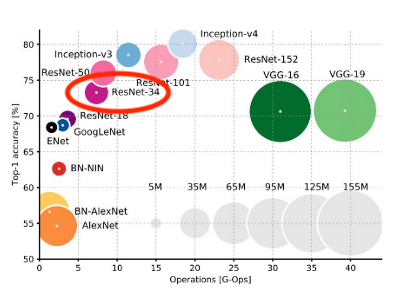
\includegraphics [scale=1] {resnet}
  \caption{Соотношение точности к сложности вычислений у ResNet-34 относительно других архитектур} 
  \label{img:resnet}  
\end{figure}

Для того чтобы гарантировать исполнение условий, указанных в содержательной постановке задачи, используется предобученная нейронная сеть по сегментации изображений MaskRCNN. Она получает на вход изображение и возвращает маску объектов, находящихся на ней. Нас интересуют собаки. Если масок несколько - значит, на кадре больше одной собаки. Если масок собак нет - значит на кадре собак нет. Эти две простые проверки сильно увеличивают качество нейронной сети. Помимо этих проверок, маска позволяет убрать ненужную часть кадра, уменьшая шанс того что нейронная сеть ошибётся.

Также в работе используется MobileNet v2\cite{mobilenet} при работе с маленькими датасетами. Изменения от оригинальной статьи только в так называемой «голове» классификации и размере входного изображения. Структура следующая:

\begin{figure}[ht] 
  \center
  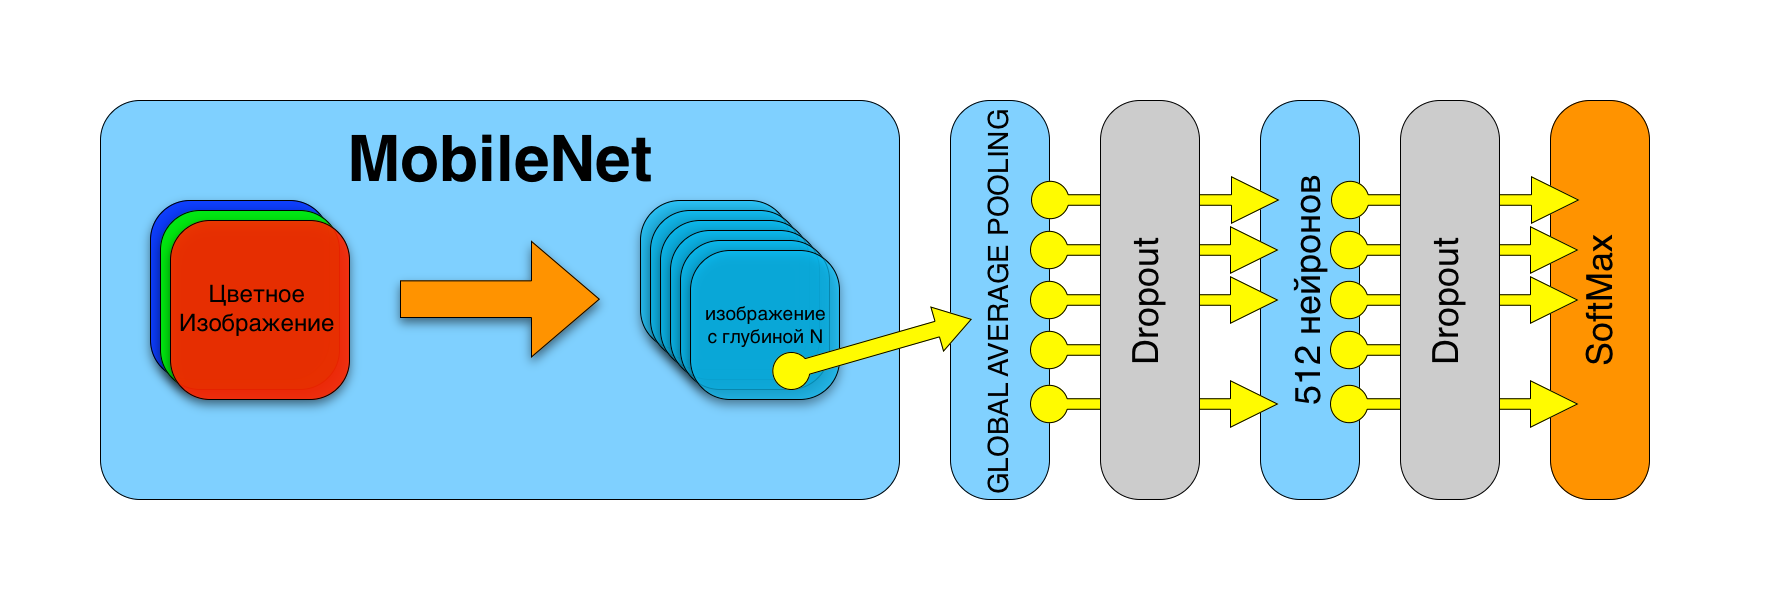
\includegraphics [width=\textwidth] {NN_arch}
  \caption{Архитектура используемой нейронной сети} 
  \label{img:NN_arch}  
\end{figure}

\begin{itemize}
    \item Входное изображение 96х96 пикселей с 3 каналами
    \item Основа MobileNet V2, без "головы"
    \item Global Average Pooling - последняя карта активации(3-мерный тензор) преобразуется в плоский вектор, каждый слой превращается в одно число - среднее по слою. Это позволяет нейронной сети быть инвариантной к размеру входного изображения
    \item Слой DropOut - обнуление 20\% разных значений предыдущего слоя
    \item Batch Norm - нормализация вектора относительно других изображений в мини-партии данных для обучения
    \item Полносвязный слой с 512 нейронами
    \item Функция активации, ReLU
    \item DropOut
    \item BatchNorm
    \item Выходной слой n нейронов, по количеству классов. Функция активации - softmax. 
\end{itemize}

Такая архитектура обусловлена борьбой с переобучением нейронной сети на маленьких объёмах данных. Размер входного изображения держался на минимальном уровне, обычно нейронные сети используют по 224 пикселя по длине и ширине, здесь же всего 96. Множественные DropOut и Batch Normalization тоже сильно мешают нейронной сети "зазубрить" датасет, так как они каждый раз немного изменяют выходы предыдущих слоёв.

Сама архитектура MobileNet тоже выбрана неслучайно. Она обладает крайне малым количеством обучаемых параметров, при этом выдаёт совершенно замечательные результаты классификации известных датасетов.\cite{mobilenet}

\begin{figure}[ht] 
  \center
  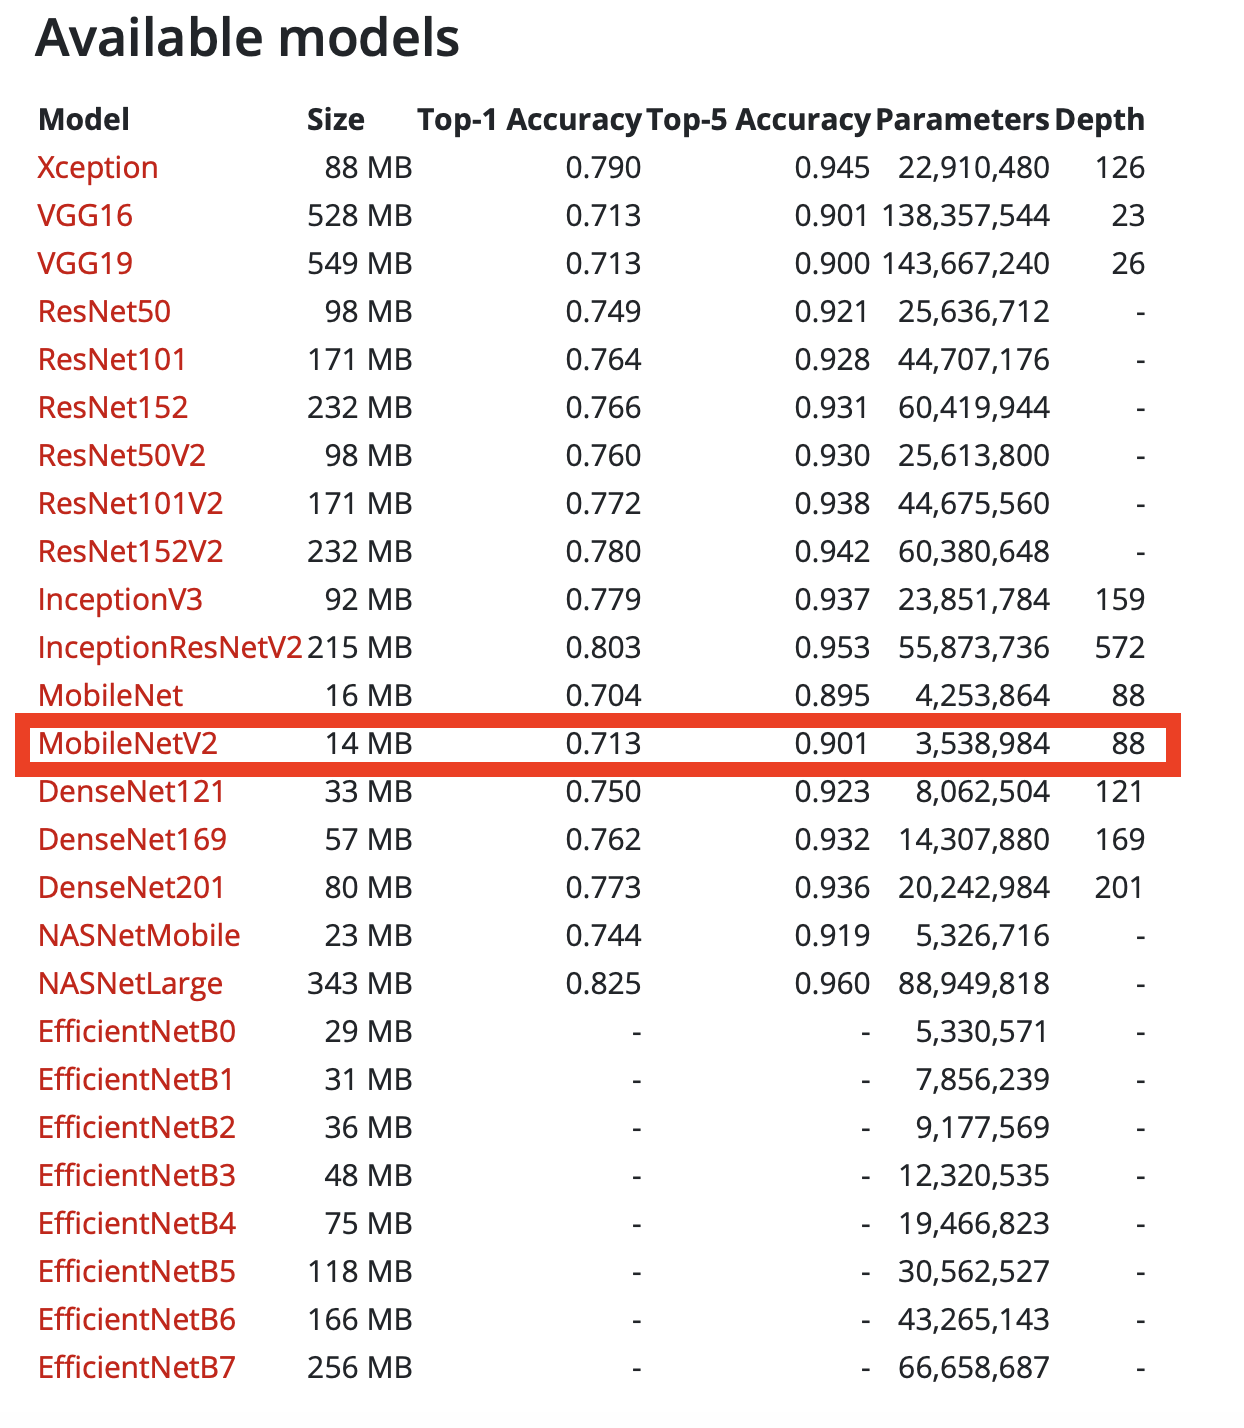
\includegraphics [width=\textwidth*2/3] {mobilenet_vs_rest}
  \caption{MobileNet обладает практически минимальным количеством обучаемых параметров, при этом не отстаёт по точности от других архитектур} 
  \label{img:resnet}  
\end{figure}

